\documentclass[a4paper]{article}

\usepackage[english]{babel}
\usepackage[utf8]{inputenc}
\usepackage{amsmath}
\usepackage{graphicx}
\usepackage[colorinlistoftodos]{todonotes}
\usepackage{amsmath}  
\newtheorem{theorem}{Theorem}  
\newtheorem{definition}{Definition}  
\newtheorem{lemma}{Lemma}  
\newtheorem{proposition}{Proposition}
\newtheorem{proof}{Proof}[section] 
\usepackage{indentfirst}
\usepackage{bbm}
\usepackage{multirow}
\advance\day by -2

\title{Problème de planification culturale durable \footnote{Ce rapport est destiné au TP7 de cours Recherche Opérationnelle et Développement Durable du programme MPRO encadré par Professeur Agnès Plateau sur le sujet de la planification culturale.}}

\author{Ling \textsc{Ma} and Changmin \textsc{Wu}}
\date{\today}

\begin{document}
\maketitle
\tableofcontents

\section{Quelques notations}
\begin{itemize}
    \item $\mathcal{T}$: $\{1, \ldots, T\}$ le horizon de planification.
    \item $\mathcal{P}$: $\{1, \ldots, P\}$ ensemble des parcelles utilisables.
    \item $s(t)$: $s(t)=1$ temps impair; $s(t)=2$ temps pair.
    \item $C(s(t))$: ensemble des cultures cultivables au temps $t$.
    \item $D_{j,t}$: demande en tonnes de culture $j$ au temps $t$.
    \item $(l,a,j)$: état d'une parcelle où
    \begin{itemize}
        \item $l$: le nombre de temps consécutifs de jachère.
        \item $a$: le nombre de temps consécutifs de culture (si $j \neq 0$).
        \item $j$: $C \cup \{0\}$ où $C$ l'ensemble des cultures cultivables et $0$ la jachère.
    \end{itemize}
    \item $(l',a',i) -> (l,a,j)$: une transition d'une parcelle d'état $(l',a',i)$ à $(l,a,j)$ qui est associé avec un rendement $\text{REND}(l,a,i,j)$.
\end{itemize}

\section{Une représentation du graphe}
Figure \ref{fig:diam} présente un tel graphe dont chaque sommet désigne un état possible de la forme $(l,a,j)$. Un chemin qui commence par $(2,0,0)$ (et de longueur $5$) est donc une rotation de $T=5$ sur la parcelle $p$, par exemple, le chemin $(2,0,0)->(2,1,R)->(2,2,H)->(1,0,0)->(1,1,H)->(1,0,0)$. 
\begin{figure}[h!t]
    \centering
    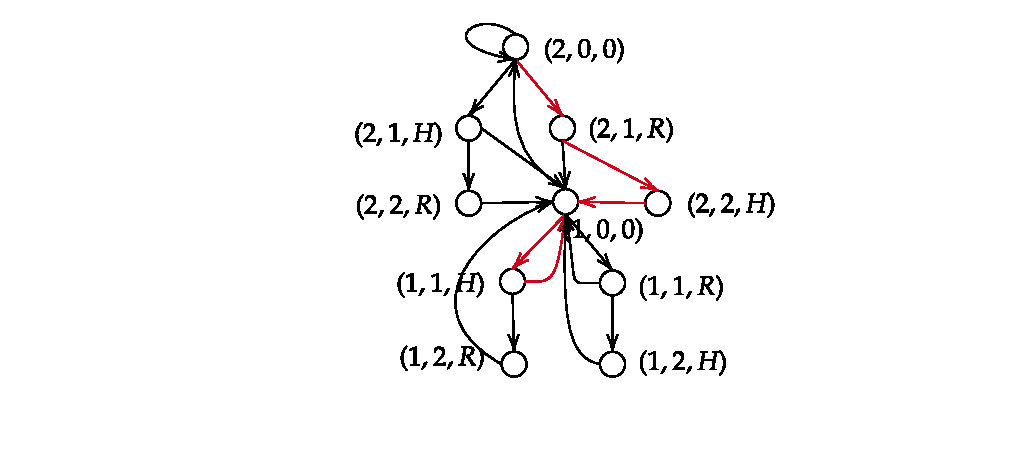
\includegraphics[width=\textwidth]{diagram.pdf}
    \caption{Graphe $G$: les arcs rouges correspondent à une rotation possible; $R$ est \textit{riz} et $H$ est \textit{haricot}}
    \label{fig:diam}
\end{figure}
Notons que chaque arc désigne une transition $(l',a',i) -> (l,a,j)$, on peut donc associer chaque arc un rendement $\text{REND}_{arc} = \text{REND}(l,arc,i,j)$ où $arc = (l',a',i) -> (l,a,j)$

\section{Modélisation PLNE}
Étant donnée la représentation du graphe, on peut modéliser ce problème de planification comme $P$ problème de flot sur $P$ graphe $G$ qui satisfit une contrainte globale. 
\begin{equation*}
    (P1) \left\{ 
    \begin{aligned}
    \min\quad        & \sum_{p\in P}\sum_{t=1}\sum_{arc \in Arcs^{-}_{(2,0,0)}} x_{p,t,arc}   \\
    \text{s.t.\quad} & \sum_{p\in P}\sum_{arc \in Arcs^{-}_{j}} \text{REND}_{arc} x_{p,t,arc} \geq D_{j,t} & & \forall t\in \mathcal{T}, j \in C(s(t)) \\
                     & \sum_{arc \in Arcs^{-}_{v}} x_{p,t,arc} = \sum_{b \in Arcs^{+}_{v}} x_{p,t+1,b} & & \forall t \in \mathcal{T}\backslash\{1,T\}, p \in \mathcal{P}, v\in V(G)\\
                     & \sum_{arc \in Arcs^{-}_{(2,0,0)}} x_{p,1,arc} \leq 1 & &  \forall p \in \mathcal{P} \\
                     & \sum_{arc \not\in Arcs^{-}_{(2,0,0)}} x_{p,1,arc} = 0 & &  \forall p \in \mathcal{P} \\
                     & x_{p,t,arc} \in \{0,1\} & & \forall t \in \mathcal{T}, p \in \mathcal{P}, arc \in Arcs
  \end{aligned}
\right.
\end{equation*}
où $x_{p,t,a}$ désigne si la transition représentée par $a$ s'effectue au temps $t$ sur la parcelle $p$. $Arc^{-}_{j}$ désigne tous arcs de $G$ incident à $j$ et $Arc^{+}_{j}$ les arcs émergent de $j$. La première contrainte est la contrainte de la demande. La deuxième contrainte est celui de la conservation du flot et les deux prochaines sont les contraintes d'état initial (tout chemin commence de $(2,0,0)$).

\section{Résultat}
Voir tableau \ref{tab:res}.
\begin{table}
    \centering
    \resizebox{1 \textwidth}{!}{
    \begin{tabular}{c|c|c}
    \hline
    Temps de calcul & Nbr Noeuds développés & Nbr Parcelles Cultivées \\
    \hline
    $2.47$s & $1344$ & $19$ \\
    \hline
    \end{tabular}}
    \caption{Information de la solution trouvée}
    \label{tab:res}
\end{table}

\section{Une ré-formulation}
Supposons que les rotations $r$ sont énumérable, et elle est représentée par une suite de transitions (arcs). on a
\begin{equation*}
    (P2) \left\{ 
    \begin{aligned}
    \min\quad        & \sum_{r \in R} x_{r}   \\
    \text{s.t.\quad} & \sum_{r \in R} A_{j,t,r} x_{r} \geq D_{j,t} & & \forall t\in \mathcal{T}, j \in C(s(t))\\
                     & x_r \in \mathbbm{Z}_+            & & \forall r
  \end{aligned}
\right.
\end{equation*}
où $r_t$ est la transition de la rotation $r$ au temps $t$, $A_{j,t,r} = \text{REND}_{r_t}$ si $r_t \in Arcs^{-}_{j}$ et $0$ autrement. 

\section{Génération de colonnes}
Quand on applique l'algorithme de la génération de colonnes, tout d'abord on cherche la solution pour le dual du programme $P2$ (ou sa relaxation) avec variables duales $z_{j,t}$. Après avec la solution trouvée de $z_{j,t}$, on cherche un nouveau colonne $A_{k}$ qui minimise le coût réduit négatif $1-\sum_{j,t} z_{j,t} A_{j,t,k}$. Donc si on associe à chaque arc de $G$ un coût de $-z_{j,t}\text{REND}_{arc}$, le problème peut être réduit à un problème du plus court chemin dans un graphe pondéré, que on peut résoudre facilement par l'algorithme de Bellman à chaque itération du processus de génération de colonnes jusqu'à où on ne peut plus trouver un chemin dont le coût réduit est négatif. 

\end{document}
